\let\negmedspace\undefined
\let\negthickspace\undefined
\documentclass[journal]{IEEEtran}
\usepackage[a5paper, margin=10mm, onecolumn]{geometry}

\setlength{\headheight}{1cm} % Set the height of the header box
\setlength{\headsep}{0mm}     % Set the distance between the header box and the top of the text

\usepackage{gvv-book}
\usepackage{gvv}
\usepackage{cite}
\usepackage{amsmath,amssymb,amsfonts,amsthm}
\usepackage{algorithmic}
\usepackage{graphicx}
\usepackage{textcomp}
\usepackage{xcolor}
\usepackage{txfonts}
\usepackage{enumitem}
\usepackage{mathtools}
\usepackage{gensymb}
\usepackage{comment}
\usepackage[breaklinks=true]{hyperref}
\usepackage{tkz-euclide} 
\usepackage{inputenc}                                
\usepackage{color}                                            
\usepackage{array}                                            
\usepackage{longtable}                                       
\usepackage{calc}                                             
\usepackage{multirow}                                         
\usepackage{hhline}                                           
\usepackage{ifthen}                                           
\usepackage{lscape}
\usepackage{tikz}
\usepackage{circuitikz}
\usepackage{standalone} % For including external TikZ files

\begin{document}

\bibliographystyle{IEEEtran}
\vspace{3cm}

\title{11.16.3.21.1}
\author{EE24BTECH11013 - MANIKANTA D}
{\let\newpage\relax\maketitle}

\renewcommand{\thefigure}{\theenumi}
\renewcommand{\thetable}{\theenumi}
\setlength{\intextsep}{10pt} % Space between text and floats

\numberwithin{equation}{enumi}
\numberwithin{figure}{enumi}
\renewcommand{\thetable}{\theenumi}

\textbf{Question:}\\
In a class of 60 students, 30 opted for NCC, 32 opted for NSS, and 24 opted for both NCC and NSS. If one of these students is selected at random, find the probability that:
\begin{enumerate}
    \item The student opted for NCC or NSS.
\end{enumerate}

\section{Theoretical Solution}
The total number of students in the class is:
\begin{align}
    |S| &= 60.
\end{align}
The number of students who opted for NCC or NSS can be calculated using the formula for the union of two sets:
\begin{align}
    |A \cup B| &= |A| + |B| - |A \cap B|.
\end{align}
where:
\begin{align}
    |A| &= 30, \quad \text{(students who opted for NCC)} \\
    |B| &= 32, \quad \text{(students who opted for NSS)} \\
    |A \cap B| &= 24, \quad \text{(students who opted for both NCC and NSS)}.
\end{align}
Substituting these values, we get:
\begin{align}
    |A \cup B| &= 30 + 32 - 24 = 38.
\end{align}
The probability of a student opting for NCC or NSS is:
\begin{align}
    P(A \cup B) &= \frac{|A \cup B|}{|S|} = \frac{38}{60} = \frac{19}{30} \approx 0.6333.
\end{align}

\section{Event Definition}
Define events as shown in Table \ref{table1}:
\begin{table}[h!]    
  \centering
  \caption{Defining Events}
  \label{table1}
  \begin{tabular}{ |c| c| } 
    \hline
    {Event} & {Denotation}\\ 
    \hline
    $A^\prime $ &  Student does not opt for NCC \\
    \hline 
    $ A $ & Student opts for NCC\\
    \hline
    $ B^\prime $ & Student does not opt for NSS\\
    \hline   
    $ B $ & Student opts for NSS \\
    \hline
  \end{tabular}
\end{table}

\begin{table}[h!]    
  \centering
  \caption{Boolean Algebra Rules}
  \label{table2}
  \begin{tabular}{ |c| c| } 
    \hline
    {Boolean Expression} & {Interpretation}\\ 
    \hline
    $A + A^\prime = 1$ & Complement Law\\
    \hline
    $AB + A^\prime B = B$ & Absorption Law\\
    \hline
    $AB + AB^\prime = A$ & Distributive Law\\
    \hline
    $A + B = AB + AB^\prime + A^\prime B$ & Union of Sets\\
    \hline
    $P(A + B) = P(A) + P(B) - P(AB)$ & Inclusion-Exclusion Principle\\
    \hline
    $P(A^\prime B^\prime) = 1 - P(A + B)$ & Complement Rule\\
    \hline
  \end{tabular}
\end{table}

\section{Boolean Algebra Principles}
Below are some axioms and theorems from Boolean algebra:\\
 For any two events A and B,
\begin{align}
	\because A + A^\prime &= 1 
    \end{align}
    \begin{align}
	 AB + A^\prime B &= B \label{2} 
     \end{align}
    \begin{align}
	 \implies \pr{AB} + \pr{A^\prime B} &= \pr{B} \label{3} 
     \end{align}

     \begin{align}
	 A + B &= AB + AB^\prime + A^\prime B 
     \end{align}
     \begin{align}
	 \pr{A + B} &= \pr{AB} + \pr{AB^\prime} + \pr{A^\prime B} 
     \end{align}
	\begin{align}
	 \pr{AB} &= \pr{A} + \pr{B} - \pr{A + B} 
     \end{align}

From the given data:
\begin{align}
    P(A) &= \frac{30}{60}, \quad
    P(B) = \frac{32}{60}, \quad
    P(AB) = \frac{24}{60}
\end{align}
Now applying probability axioms:
\begin{align}
    P(A + B) &= P(A) +  P(B) - P(A B) \\
              &= \frac{30}{60} + \frac{32}{60} - \frac{24}{60} \\
              &= \frac{38}{60} = \frac{19}{30} = 0.6333
\end{align}

\begin{figure}[h]
    \centering
    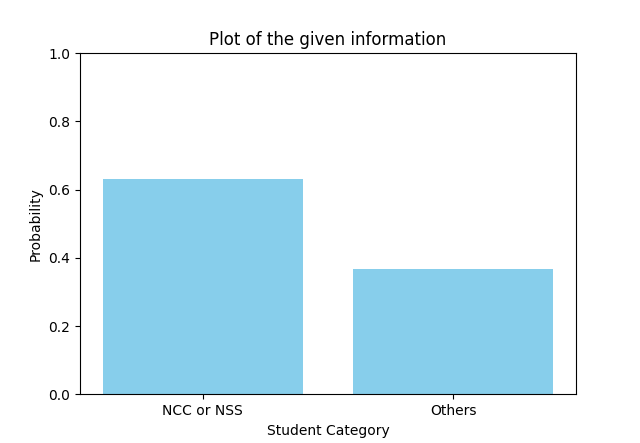
\includegraphics[width=\columnwidth]{figs/fig.png}
    \caption{Probability of opting for NCC or NSS using Boolean logic}
    \label{fig:Plot}
\end{figure}

\end{document}
 
